\clearpage
\subsubsection{Lacustrine}
\begin{table}[h!]
\centering
\caption{Categorised GPR profile keywords for lacustrine environments. Geometry, reflectivity and continuity are shown in separate columns.}
\begin{tabular}{|p{4.5cm}|p{4.5cm}|p{4.5cm}|}
\hline
\textbf{Geometry / Structure} & \textbf{Continuity} & \textbf{Amplitude / Reflectivity} \\
\hline
Mounded & Continuous & Medium amplitude \\
Downlap & Semi-continuous & High amplitude \\
Dipping & Discontinuous & Low amplitude \\
Lenticular & Wavy & High reflectivity \\
Concave & & Low reflectivity \\
Layered & & Varied reflectivity \\
Oblique & & High attenuation \\
Wedge & & \\
Prograding & & \\
Clinoform & & \\
Sigmoidal & & \\
Horizontal & & \\
Parallel & & \\
Subparallel & & \\
Foreset truncation & & \\
Sub-horizontal & & \\
\hline
\end{tabular}
\label{tab:lacustrine-keywords}
\end{table}

\begin{figure}[h!]
    \centering
    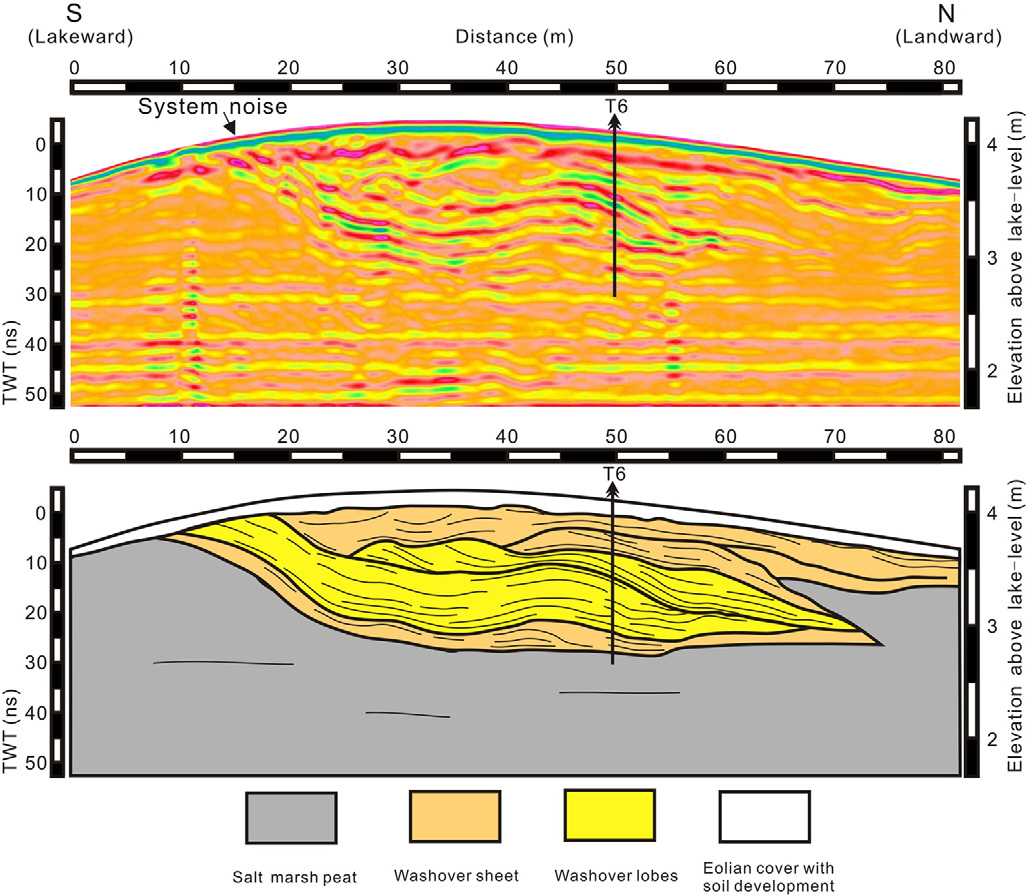
\includegraphics[width=0.9\linewidth]{Figures/0.2GPR/Shan2015_fill_3.png}
    \caption[Shore-parallel profile of trenches (1).]{Shore-parallel profile of trenches (1).\textbf{Keywords: } Mounded, downlap, dipping, lenticular, concave, layered, continuous, semi-continuous, discontinuous, medium amplitude, high amplitude, high reflectivity, low reflectivity \citep{Shan2015}.}
    \label{fig:Shan2015-3}
\end{figure}
\begin{figure}[h!]
    \centering
    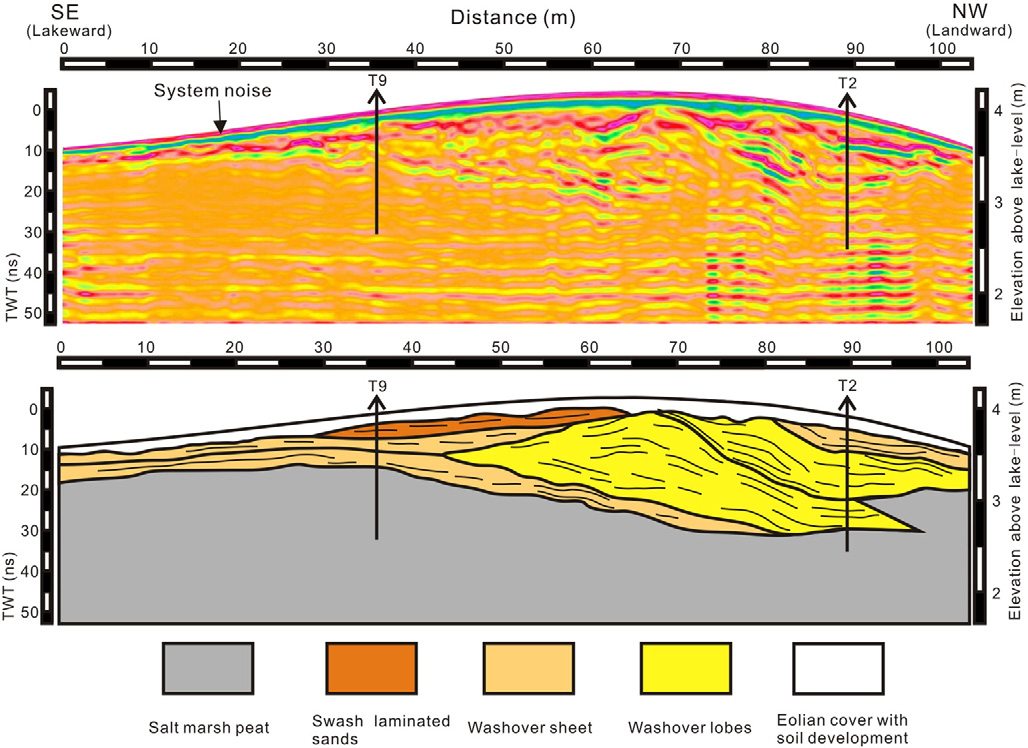
\includegraphics[width=0.9\linewidth]{Figures/0.2GPR/Shan2015_fill_4.png}
    \caption[Shore-parallel profile of trenches (2).]{Shore-parallel profile of trenches (2). \textbf{Keywords: } Oblique, wedge, concave, semi-continuous, wavy, discontinuous, high amplitude, low amplitude, varied reflectivity\citep{Shan2015}.}
    \label{fig:Shan2015-4}
\end{figure}

\begin{figure}[h!]
    \centering
    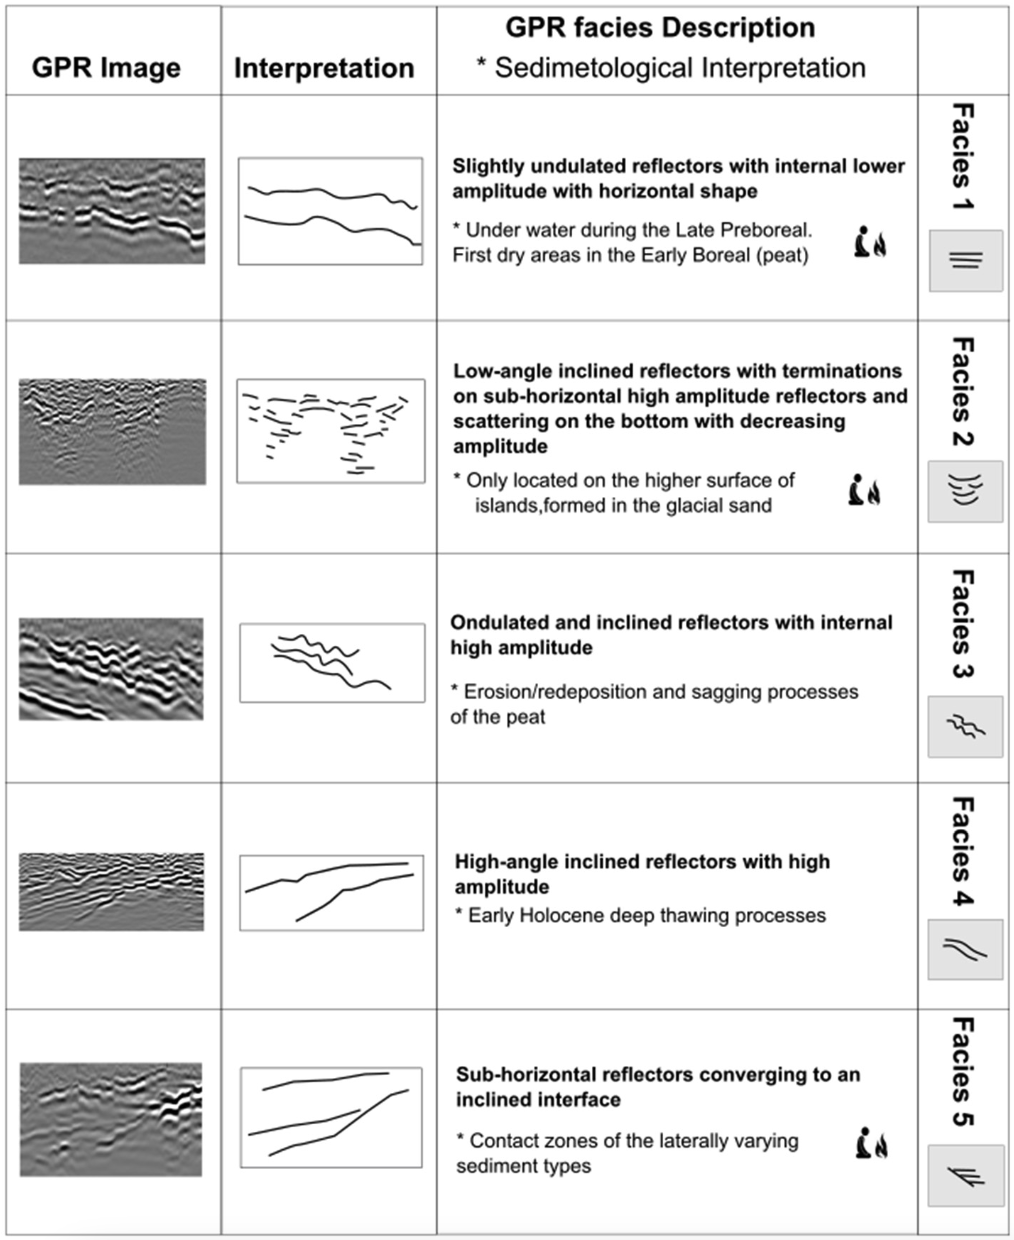
\includegraphics[width=0.9\linewidth]{Figures/0.2GPR/Corradini_2023_lake_bog.png}
    \caption[Lake and bog.]{Lake and bog. \textbf{Keywords: } Low amplitude, discontinuous, dipping, high amplitude, high attenuation, sub-horizontal \citep{Corradini2023}.}
    \label{fig:Corradini2023-1}
\end{figure}

\begin{figure}[h!]
    \centering
    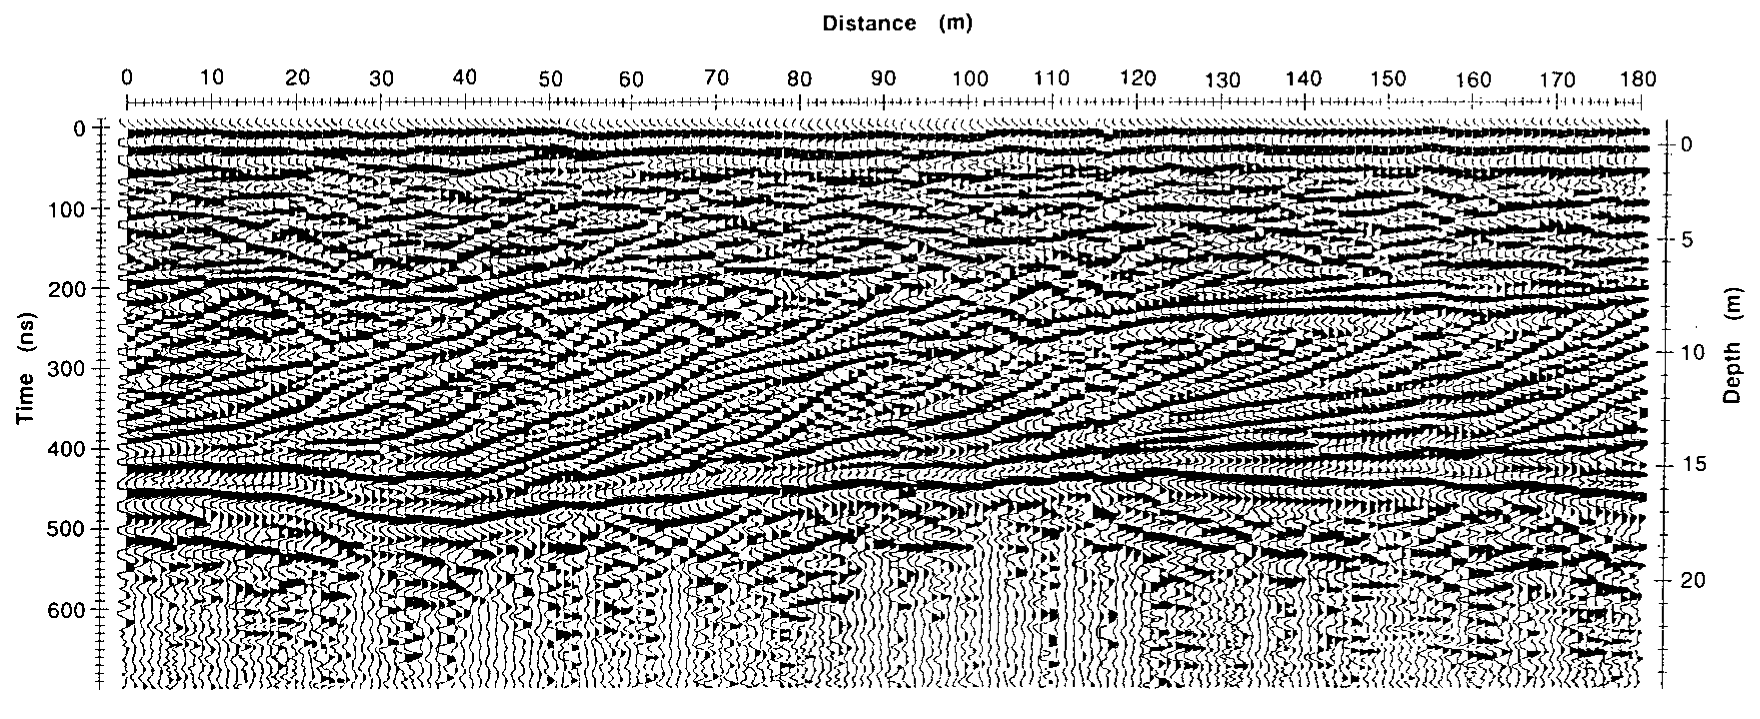
\includegraphics[width=0.9\linewidth]{Figures/0.2GPR/Jol1991_1.png}
    \caption[Lacustrine delta (1).]{Lacustrine delta (1). \textbf{Keywords: } Prograding, clinoform, downlap, sigmoidal, continuous, horizontal, dipping, high attenuation \citep{Jol1991-1}.}
    \label{fig:Jol1991-1}
\end{figure}

\begin{figure}[h!]
    \centering
    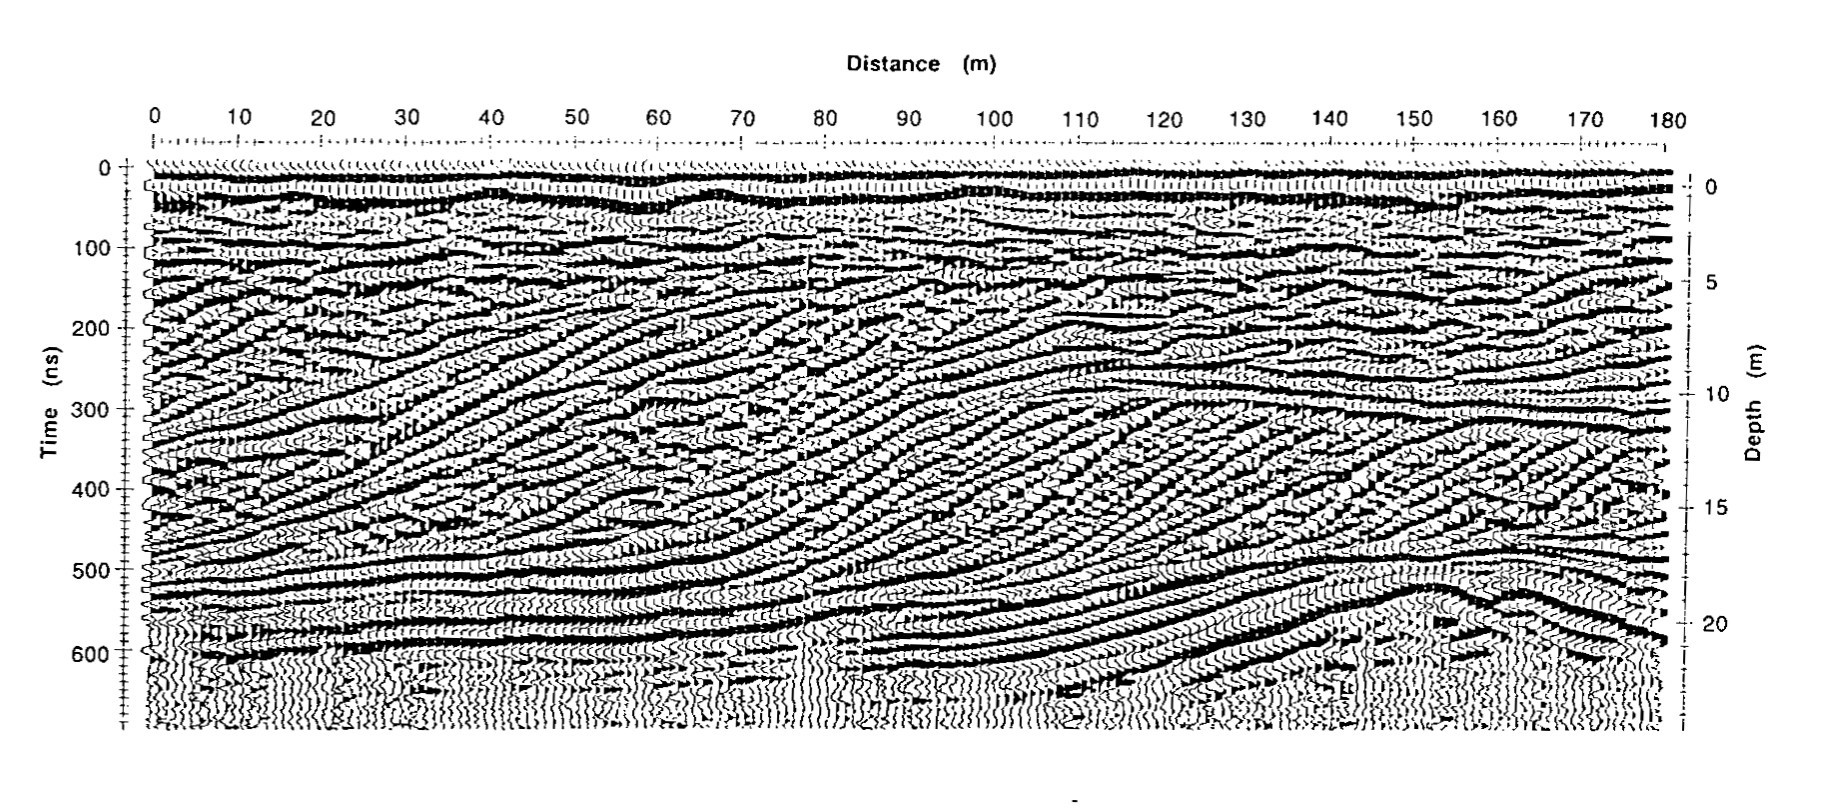
\includegraphics[width=0.9\linewidth]{Figures/0.2GPR/Jol1991_2_1.png}
    \caption[Lacustrine delta (2).]{Lacustrine delta (2). \textbf{Keywords: } Clinoform, downlap, dipping, parallel, subparallel topset, continuous, prograding, foreset truncation, high attenuation \citep{Jol1991-1}.}
    \label{fig:Jol1991-2-1}
\end{figure}